
\documentclass{article}
\usepackage{geometry} 
\usepackage{booktabs}         %for tables
%\geometry{letterpaper} 
\usepackage{graphicx}
\usepackage{amssymb}
\usepackage{hyperref}         %use hyperlink
\usepackage{epstopdf}
\DeclareGraphicsRule{.tif}{png}{.png}{`convert #1 `dirname #1`/`basename #1 .tif`.png}
\makeatletter
\def\verbatim@font{\ttfamily\scriptsize}
\makeatother
\begin{document}


\section{Introduction to MarkDoc (heading
1)}\label{introduction-to-markdoc-heading-1}

\subsection{Using Markdown (heading 2)}\label{using-markdown-heading-2}

Writing with \textbf{markdown} syntax allows you to add text and graphs
to \emph{smcl} logfile and export it to a editable document format. I
will demonstrate the process by using the \textbf{Auto.dta} dataset.

\subsubsection{Get started with MarkDoc (heading
3)}\label{get-started-with-markdoc-heading-3}

I will open the dataset, list a few observations, and export a graph.
Then I will export the logfile to Microsoft Office docx format.

\paragraph{Even smaller bolding}\label{even-smaller-bolding}

\emph{italics}

\emph{one underscore} is probably \emph{also} italics.

\begin{verbatim}
      . sysuse auto, clear
      
      .       histogram price
      (bin=8, start=3291, width=1576.875)
      
      
      .      graph export graph.png,  width(400) replace
      (file graph.png written in PNG format)
      
      
\end{verbatim}

You use two stars to include only output, and three stars to include
only the command. So two stars plus ``quietly'' gets you nothing. You
can also add numbers inline, but it's not quite as smooth as in R
Markdown.

Because you put it on the next command line to say the mean of Price
variable is 6165.26 and SD is 2949.50

\section{Adding a graph or image in the
report}\label{adding-a-graph-or-image-in-the-report}

\subsection{Adding a graph using
Markdown}\label{adding-a-graph-using-markdown}

In order to add a graph using Markdown, I export the graph in PNG
format. You can explain the graph in the ``brackets'' and define the
file path in parentheses

\begin{figure}[htbp]
\centering
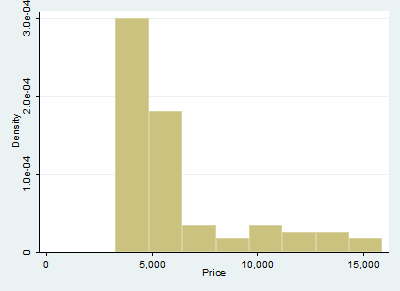
\includegraphics{./graph.png}
\caption{explain the graph}
\end{figure}

You can also export to a ton of different file types. (Thanks, pandoc!)
So that's actuall y kind of cool.

Let's try and add math at the bottom. \(y_i=\alpha+\beta_1*X_i\)

\end{document}



